\section{14 Sept 23 - Conducting a complete analysis of an
ODE}\label{sept-23---conducting-a-complete-analysis-of-an-ode}

We've built up all the tools that we use to investigate ODEs. Now we are
going to practice with an oscillator that exhibits really interesting
dynamics: the
\href{https://en.wikipedia.org/wiki/Van_der_Pol_oscillator}{Van der Pol
oscillator}. This equation originates from nonlinear circuits in early
radios, but has now also been used in neuroscience and geology. It is
given by the differential equation:

\[
\ddot{x} = -\mu (x^2 - 1)\dot{x} - x
\]

or, written as two first order equations:

\[
\dot{x} = v \hspace{1in} \dot{v} = -\mu (x^2 - 1)v - x
\]

With \(\mu > 0\). Note that this equation is simply the harmonic
oscillator when \(\mu = 0\). The strange \(-\mu (x^2 - 1)\dot{x}\)
represents damping, but this damping behaves strangely, because when
\(|x|<1\) it is negative damping, that is it boosts oscillations smaller
than \(1\), while still slowing down oscillations larger than \(1\).

Now we play the usual game of trying to figure out how this system
behaves:

\textbf{✅ Do this}

\begin{enumerate}
\def\labelenumi{\arabic{enumi}.}
\tightlist
\item
  Identify the fixed point of this system. Follow the linearization
  procedure to characterize it.
\item
  Edit the code below to produce a phase plot for the Van der Pol
  oscillator. This code also numerically integrates a trajectory and
  plots it. Add a second trajectory and plot that as well.
\item
  What happens to phase space when you change the value of \(\mu\)? What
  if you make it negative?
\item
  What behavior do you notice here that's different than you've seen
  before? What is attracting the trajectories?
\end{enumerate}

\begin{Shaded}
\begin{Highlighting}[]
\ImportTok{import}\NormalTok{ numpy }\ImportTok{as}\NormalTok{ np}
\ImportTok{import}\NormalTok{ matplotlib.pyplot }\ImportTok{as}\NormalTok{ plt}
\ImportTok{from}\NormalTok{ scipy.integrate }\ImportTok{import}\NormalTok{ solve\_ivp}

\KeywordTok{def}\NormalTok{ VP\_eqn(x, v, mu }\OperatorTok{=} \FloatTok{1.}\NormalTok{):}
\NormalTok{    xdot, vdot }\OperatorTok{=}\NormalTok{ [}\DecValTok{0}\NormalTok{,}\DecValTok{0}\NormalTok{] }\CommentTok{\#\# CHANGE}
    \ControlFlowTok{return}\NormalTok{ xdot, vdot}

\KeywordTok{def}\NormalTok{ VP\_phase(X, VX, mu):}
\NormalTok{    xdot, vdot }\OperatorTok{=}\NormalTok{ np.zeros(X.shape), np.zeros(VX.shape)}
\NormalTok{    Xlim, Ylim }\OperatorTok{=}\NormalTok{ X.shape}
    \ControlFlowTok{for}\NormalTok{ i }\KeywordTok{in} \BuiltInTok{range}\NormalTok{(Xlim):}
        \ControlFlowTok{for}\NormalTok{ j }\KeywordTok{in} \BuiltInTok{range}\NormalTok{(Ylim):}
\NormalTok{            xloc }\OperatorTok{=}\NormalTok{ X[i, j]}
\NormalTok{            yloc }\OperatorTok{=}\NormalTok{ VX[i, j]}
\NormalTok{            xdot[i,j], vdot[i,j] }\OperatorTok{=}\NormalTok{ VP\_eqn(xloc, yloc,mu)}
    \ControlFlowTok{return}\NormalTok{ xdot, vdot}

\KeywordTok{def}\NormalTok{ VP\_eqn\_for\_solve\_ivp(t,curr\_vals, mu}\OperatorTok{=}\DecValTok{1}\NormalTok{): }\CommentTok{\# need to rephrase this to work with what solve\_ivp expects}
\NormalTok{    x, v }\OperatorTok{=}\NormalTok{ curr\_vals }
\NormalTok{    xdot, vdot }\OperatorTok{=}\NormalTok{ VP\_eqn(x,v,mu)}
    \ControlFlowTok{return}\NormalTok{ xdot,vdot}

\CommentTok{\# Numerical Integration}
\NormalTok{tmax }\OperatorTok{=} \DecValTok{20}
\NormalTok{dt }\OperatorTok{=} \FloatTok{0.05}
\NormalTok{tspan }\OperatorTok{=}\NormalTok{ (}\DecValTok{0}\NormalTok{,tmax)}
\NormalTok{t }\OperatorTok{=}\NormalTok{ np.arange(}\DecValTok{0}\NormalTok{,tmax,dt)}
\NormalTok{mu }\OperatorTok{=} \FloatTok{1.}
\NormalTok{initial\_condition }\OperatorTok{=}\NormalTok{ [}\DecValTok{1}\NormalTok{, }\DecValTok{1}\NormalTok{] }
\NormalTok{solved }\OperatorTok{=}\NormalTok{ solve\_ivp(VP\_eqn\_for\_solve\_ivp,tspan,initial\_condition,t\_eval }\OperatorTok{=}\NormalTok{ t, args }\OperatorTok{=}\NormalTok{ (mu,),method}\OperatorTok{=}\StringTok{"RK45"}\NormalTok{)}


\CommentTok{\# Plotting stuff}
\NormalTok{N }\OperatorTok{=} \DecValTok{40}
\NormalTok{x }\OperatorTok{=}\NormalTok{ np.linspace(}\OperatorTok{{-}}\FloatTok{3.}\NormalTok{, }\FloatTok{3.}\NormalTok{, N)}
\NormalTok{v }\OperatorTok{=}\NormalTok{ np.linspace(}\OperatorTok{{-}}\FloatTok{3.}\NormalTok{, }\FloatTok{3.}\NormalTok{, N)}
\NormalTok{X, V }\OperatorTok{=}\NormalTok{ np.meshgrid(x, v)}
\NormalTok{xdot, vdot }\OperatorTok{=}\NormalTok{ VP\_phase(X, V,mu)}
\NormalTok{ax }\OperatorTok{=}\NormalTok{ plt.figure(figsize}\OperatorTok{=}\NormalTok{(}\DecValTok{10}\NormalTok{,}\DecValTok{10}\NormalTok{))}
\NormalTok{Q }\OperatorTok{=}\NormalTok{ plt.streamplot(X, V, xdot, vdot, color}\OperatorTok{=}\StringTok{\textquotesingle{}k\textquotesingle{}}\NormalTok{,broken\_streamlines }\OperatorTok{=} \VariableTok{False}\NormalTok{)}
\NormalTok{plt.plot(solved.y[}\DecValTok{0}\NormalTok{],solved.y[}\DecValTok{1}\NormalTok{],lw }\OperatorTok{=} \DecValTok{3}\NormalTok{,c }\OperatorTok{=} \StringTok{\textquotesingle{}red\textquotesingle{}}\NormalTok{) }\CommentTok{\# plot trajectory from solve\_ivp}
\NormalTok{plt.grid()}
\NormalTok{plt.xlabel(}\StringTok{\textquotesingle{}$x$\textquotesingle{}}\NormalTok{)}
\NormalTok{plt.ylabel(}\StringTok{\textquotesingle{}$v$\textquotesingle{}}\NormalTok{)}
\NormalTok{plt.show()}
\end{Highlighting}
\end{Shaded}

\begin{figure}
\centering
\pandocbounded{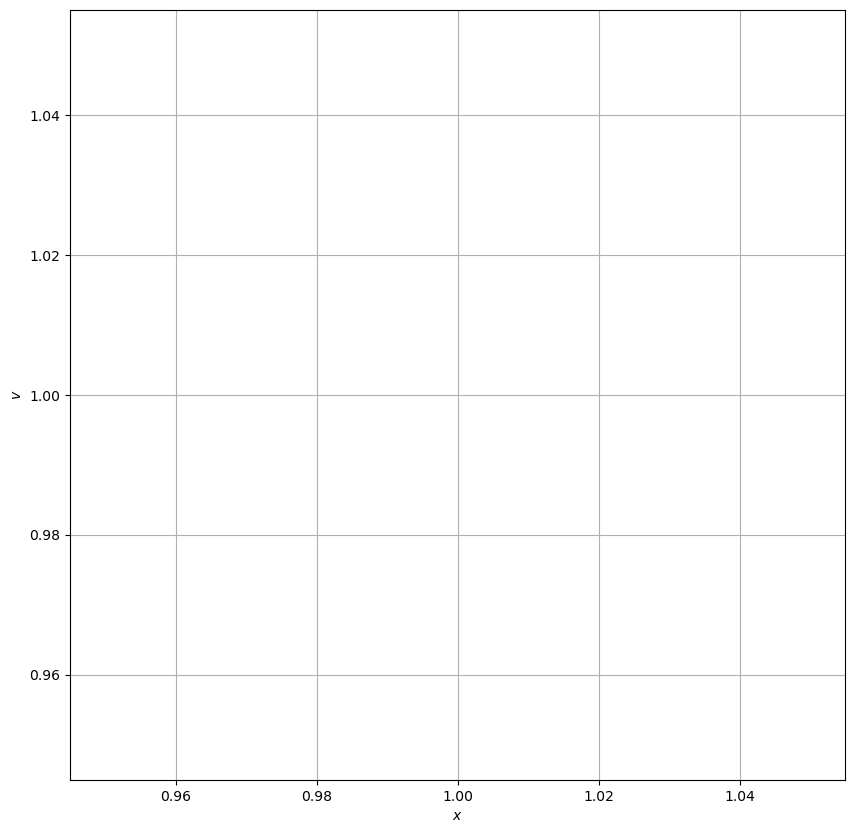
\includegraphics[keepaspectratio,alt={png}]{../images/activity_vanderpol_activity_vanderpol_tmp_1_0.png}}
\caption{png}
\end{figure}

\textbf{✅ Do this}

Based on the phase space diagram, what do you expect actual trajectories
to look like in \(x\) vs \(t\) space? Use the numerically integrated
trajectories to plot that.

\begin{Shaded}
\begin{Highlighting}[]

\end{Highlighting}
\end{Shaded}

\subsection{Limit Cycles}\label{limit-cycles}

The new behavior we've seen from this equation is what's called a
\textbf{limit cycle}, where the system is attracted/reppeled from a
closed curve instead of a fixed point(s). There's a lot of really great
math here that's a bit beyond what we can cover in class, but it would
be a great thing to look into for a project!

\textbf{✅ Do this}

Spend the rest of class investigating the Van der Pol oscillator. Here
are a few investigations you could do:

\begin{itemize}
\tightlist
\item
  When \(\mu\) changes from negative to positive, this system undergoes
  what is known as a \textbf{Hopf Bifurcation} Look up what bifurcations
  are to understand what this means and show that it is true using
  numerical integration.
\item
  Add an \(A\sin(t)\) driving force term to the differential equation
  and numerically integrate. What do these trajectories look like in
  \(x\) vs \(t\) and in phase space?
\item
  Examine the energetics of this system. Is energy conserved or does it
  have some interesting behavior? Why?
\end{itemize}
